\documentclass[tikz,border=10pt]{standalone}
\usepackage{tikz}
\usetikzlibrary{calc}
\definecolor{aksen}{HTML}{F7B538}
\definecolor{latar}{HTML}{171D2B}
\newcommand{\buku}{%
  \tikz{\fill[aksen!80,draw=white,thick]
    (-0.35,-0.45) rectangle (0.35,0.45);
    \draw[white,thick] (0,-0.45) -- (0,0.45);}}
\newcommand{\setengahbuku}{%
  
\begin{tikzpicture}
    \begin{scope}
      \clip (-0.5,-0.6) rectangle (0,0.6);
      \fill[aksen!80,draw=white,thick]
        (-0.35,-0.45) rectangle (0.35,0.45);
      \draw[white,thick] (0,-0.45) -- (0,0.45);
    \end{scope}
  \end{tikzpicture}}
\begin{document}
\pagecolor{latar}
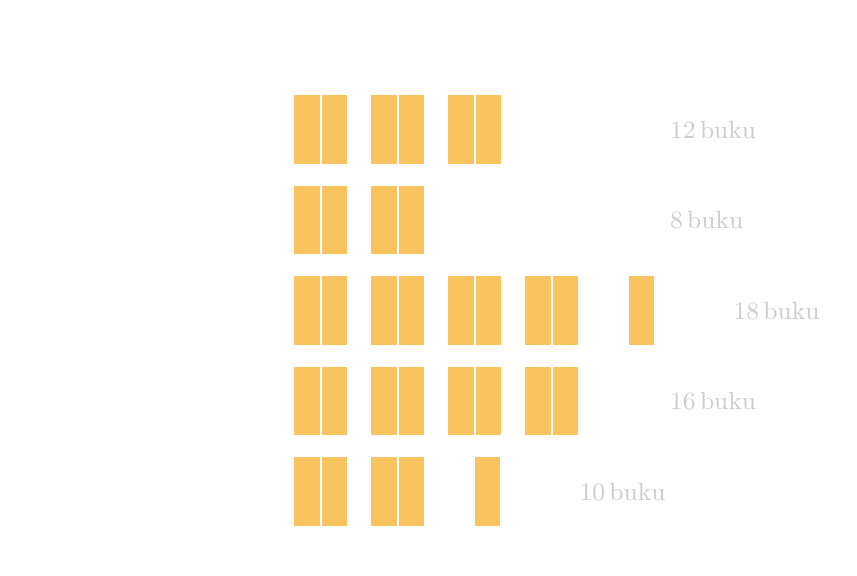
\begin{tikzpicture}[scale=1.15, text=white,
  hari/.style={anchor=east, font=\bfseries},
  jumlah/.style={anchor=west, font=\small}]
  % Senin 12/3, Selasa 8/2, Rabu 18/4.5, Kamis 16/4, Jumat 10/2.5
  \node[hari] at (-1.2, -0) {Senin};
  \node at (0.85,-0) {\buku}; \node at (1.7,-0) {\buku}; \node at (2.55,-0) {\buku};
  \node[jumlah, gray!40] at (4.6, -0) {12\,buku};

  \node[hari] at (-1.2, -1) {Selasa};
  \node at (0.85,-1) {\buku}; \node at (1.7,-1) {\buku};
  \node[jumlah, gray!40] at (4.6, -1) {8\,buku};

  \node[hari] at (-1.2, -2) {Rabu};
  \node at (0.85,-2) {\buku}; \node at (1.7,-2) {\buku};
  \node at (2.55,-2) {\buku}; \node at (3.4,-2) {\buku};
  \node[anchor=west] at (4.0,-2) {\setengahbuku};
  \node[jumlah, gray!40] at (5.3, -2) {18\,buku};

  \node[hari] at (-1.2, -3) {Kamis};
  \node at (0.85,-3) {\buku}; \node at (1.7,-3) {\buku};
  \node at (2.55,-3) {\buku}; \node at (3.4,-3) {\buku};
  \node[jumlah, gray!40] at (4.6, -3) {16\,buku};

  \node[hari] at (-1.2, -4) {Jumat};
  \node at (0.85,-4) {\buku}; \node at (1.7,-4) {\buku};
  \node[anchor=west] at (2.3,-4) {\setengahbuku};
  \node[jumlah, gray!40] at (3.6, -4) {10\,buku};

  \node[anchor=west, font=\small\itshape] at (-1.2, 0.9)
    {1 gambar buku = 4 data};
\end{tikzpicture}
\end{document}
